\documentclass[]{article}
\newcommand{\FileDepth}{../../..}
\usepackage[letterpaper, landscape, margin=0.5cm]{geometry}
\usepackage[T1]{fontenc}
\usepackage{textcomp}%Not strictly necessary, but gives \textmu command for "micro."
\usepackage{fancyhdr}
\usepackage{amsmath}
\usepackage{amssymb}
\usepackage{graphicx}
\usepackage{xcolor}
\usepackage{tikz}
\usetikzlibrary{calc}
\usepackage[shortlabels]{enumitem}
\usepackage{multicol}
\usepackage{vwcol}
\usepackage{hyperref}
\usepackage{wrapfig}
\usepackage{soul}
%opening
\newcommand{\SecType}{S}
\newcommand{\Week}{5}
\title{PH 211 Studio \Week}
\author{Benjamin Bauml}
\date{Summer 2024}

\newcommand{\Purpose}{4}
\newcommand{\DefOnly}{0}

% Version 2024-06-14
% Changes
% 2024-02-21 Added xstring package to enable smooth implementation of new \ModePage command.
% 2024-04-27 Set up to split activities and formatting aspects into separate files. Removed dependence on xcomment. Added an automatic counter to number the activities in a problem set.
% 2024-05-19 Revised old format for \TeachingTips command, which did not support \DefOnly.
% 2024-06-14 Added Repurpose environment to allow mixing of different purpose levels in the same document.
\usepackage{tcolorbox}
\usepackage{xstring}
% You will want the following four lines in your document (the last two uncommented):
% For Assignment, leave Purpose as 1. For Worksheet, set to 2. For Student Solution, set to 3. For Teacher Solution, set to 4.
% If you want keep the pieces from being called manually, set DefOnly to 0.
%\newcommand{\Purpose}{4}
%\newcommand{\DefOnly}{1}
\newcommand{\Exclusion}{0}
\newcommand{\PageTurn}{0}
\newcommand{\GrayProb}{0}
\newcommand{\Tipsy}{0}

% Assignment
\if\Purpose1
\renewcommand{\Exclusion}{1}
\fi
% Worksheet
\if\Purpose2
\renewcommand{\Exclusion}{1}
\renewcommand{\PageTurn}{1}
\fi
% Student Solution
\if\Purpose3
\renewcommand{\PageTurn}{1}
\renewcommand{\GrayProb}{1}
\fi
% Teaching Copy
\if\Purpose4
\renewcommand{\PageTurn}{1}
\renewcommand{\GrayProb}{1}
\renewcommand{\Tipsy}{1}
\fi

\newenvironment{Repurpose}[1]{
\renewcommand{\Purpose}{#1}
\renewcommand{\Exclusion}{0}
\renewcommand{\PageTurn}{0}
\renewcommand{\GrayProb}{0}
\renewcommand{\Tipsy}{0}
% Assignment
\if\Purpose1
\renewcommand{\Exclusion}{1}
\fi
% Worksheet
\if\Purpose2
\renewcommand{\Exclusion}{1}
\renewcommand{\PageTurn}{1}
\fi
% Student Solution
\if\Purpose3
\renewcommand{\PageTurn}{1}
\renewcommand{\GrayProb}{1}
\fi
% Teaching Copy
\if\Purpose4
\renewcommand{\PageTurn}{1}
\renewcommand{\GrayProb}{1}
\renewcommand{\Tipsy}{1}
\fi
}{}

\def \NewQ {0}
\def \PForce {0}
\newcommand{\MaybePage}[1]{
	\def \PForce {#1}
	\if\PForce1
	\newpage
	\else
	\if\NewQ0
	\gdef \NewQ {\PageTurn}
	\else
	\newpage
	\fi
	\fi
}

\newcommand{\ModePage}[1]{
	\IfSubStr{#1}{\Purpose}{\newpage}{}
}

\newcounter{ActNumber}
\setcounter{ActNumber}{0}

\newcommand{\Problem}[4][0]{%The first argument is optional, and if it is set to 1, the \newpage will be forced. The second argument is the name of the activity, the third is the command the activity is stored as, and the fourth is the actual problem statement.
\newcommand{#3}{
\MaybePage{#1}
\addtocounter{ActNumber}{1}
\section*{\SecType\Week-\theActNumber: #2}
\if\GrayProb1
\begin{tcolorbox}[colback=lightgray,colframe=lightgray,sharp corners,boxsep=1pt,left=0pt,right=0pt,top=0pt,bottom=0pt,after skip=2pt]
\else
\begin{tcolorbox}[colback=white,colframe=white,sharp corners,boxsep=1pt,left=0pt,right=0pt,top=0pt,bottom=0pt,after skip=2pt]
\fi
#4
\end{tcolorbox}\noindent
}
\if\DefOnly0
\else
#3
\fi
}
	
\newcommand{\ProblemSub}[3][0]{%The first argument is optional, and if a string of numbers is entered into it, it will force a \newpage in any \Purpose that shows up in the string. For example, "13" would lead to the newpage being forced in modes 1 and 3. The second is the command the activity is stored as, and the third is the actual problem statement.
\newcommand{#2}{
\ModePage{#1}
\if\GrayProb1
\begin{tcolorbox}[colback=lightgray,colframe=lightgray,sharp corners,boxsep=1pt,left=0pt,right=0pt,top=0pt,bottom=0pt,after skip=2pt]
\else
\begin{tcolorbox}[colback=white,colframe=white,sharp corners,boxsep=1pt,left=0pt,right=0pt,top=0pt,bottom=0pt,after skip=2pt]
\fi
#3
\end{tcolorbox}\noindent
}
\if\DefOnly0
\else
#2
\fi
}
		
\newcommand{\Solution}[2]{%The first argument is the command the solution is stored as, and the second is the actual solution.
\newcommand{#1}{
\if\Exclusion0
#2
\fi
}
\if\DefOnly0
\else
#1
\fi
}
		
\newcommand{\ProblemFig}[2]{%The first argument is the command the figure is stored as, and the second is the actual figure.
\newcommand{#1}{
\begin{figure}[h]
#2
\end{figure}
}
\if\DefOnly0
\else
#1
\fi
}

\newcommand{\TeachingTips}[2]{%The first argument is the command the tip is stored as, and the second is the actual tip.
\newcommand{#1}{
\if\Tipsy1
\begin{tcolorbox}[colback=lightgray,colframe=black]
#2
\end{tcolorbox}
\fi
}
\if\DefOnly0
\else
#1
\fi
}
\usepackage[absolute]{textpos}
% This package relies on Assignment Format 2024-06-14 or later to work. It is recommended that the Purpose and DefOnly commands be given as such:
%\newcommand{\Purpose}{4}
%\newcommand{\DefOnly}{0}
% Activities need to be entered outside of the TeacherMargin and PresentSpace environments, otherwise they will be defined only locally. They can even go in the preamble.
\newenvironment{TeacherMargin}{\begin{textblock*}{10.8cm}(0.5cm,0.5cm)
\small}{\end{textblock*}
\hspace{0.1cm}}
\newenvironment{PresentSpace}{\begin{textblock*}{0.3cm}(26.85cm,9.35cm)
--
\end{textblock*}
\begin{textblock*}{0.3cm}(26.85cm,18.7cm)
--
\end{textblock*}
\begin{textblock*}{0.3cm}(26.85cm,12.24cm)
	--
\end{textblock*}
\begin{textblock*}{15.6cm}(11.8cm,0.5cm)
\begin{Repurpose}{1}
\Large}{\end{Repurpose}
\end{textblock*}
\hspace{0.1cm}}

\newcommand{\FBDaxes}[3]{
	\begin{scope}[shift={(#1)},rotate=#2]
		% x-axis
		\draw[thick,->] (-2,0) -- (2,0);
		\node[anchor=west] at (2,0) {$x$};
		% y-axis
		\draw[thick,->] (0,-2) -- (0,2);
		\node[anchor=west] at (0,2) {$y$};
		\coordinate (#3) at (0,0);
	\end{scope}
}
\newcommand{\FBDvectorMA}[4]{
	\begin{scope}[shift={(#1)}]
		\coordinate (#4tip) at ({#2*cos(#3)},{#2*sin(#3)});
		\draw[ultra thick,blue,->] (#1) -- (#4tip);
	\end{scope}
}
\newcommand{\FBDvectorXY}[3]{
	\begin{scope}[shift={(#1)}]
		\coordinate (#3tip) at (#2);
		\draw[ultra thick,blue,->] (0,0) -- (#3tip);
	\end{scope}
}
\newcommand{\FBDdot}[1]{
	\filldraw[black] (#1) circle (3pt);
}
%\newcommand{\MVec}[3][0]{%Creates a momentum vector of length #3 centered at #2 and rotated #1 degrees counterclockwise.
	\begin{scope}[rotate=#1,shift={(#2)}]
		\draw[->,thick] ({-#3/2},0) -- ({#3/2},0);
	\end{scope}
}
\newcommand{\MDot}[1]{%Creates a dot at #1 to represent a zero vector.
	\filldraw (#1) circle (1pt);
}
\newcommand{\MVDRows}[2][4.5]{%Creates the rows (initial, delta, final) of a momentum vector diagram. The optional argument determines the width of the table, and defaults to a good length for three columns (two objects and the total system). The non-optional argument gives a coordinate name (not displayed) to the diagram.
	\begin{scope}
		%\draw[thick] (0,5.5) -- (0,0);
		\draw[thick] (-1,4.5) -- (#1,4.5);
		\node at (-0.5,3.75) {$\vec{p}_{i}$};
		\draw[thick] (-1,3) -- (#1,3);
		\node at (-0.5,2.25) {$\Delta\vec{p}$};
		\draw[thick] (-1,1.5) -- (#1,1.5);
		\node at (-0.5,0.75) {$\vec{p}_{f}$};
		\coordinate (#2) at (0,5);
	\end{scope}
}
\newcommand{\MVDCol}[4][0.75]{%Creates a column for an object in a momentum vector diagram. The first (non-optional) argument is the coordinate name (not displayed) of the column, while the second is the displayed column header. The first argument also names the three entries down the column. The third argument anchors the column, so it should either be the coordinate name of the MVD (for the first column) or the coordinate name of the previous column. The optional argument indicates how far the center of the column should be from the previous column's edge, and defaults to 0.75
	\begin{scope}[shift={(#4)}]
		\node at (#1,0) {#3};
		%\draw[thick] ({#1*2},0.5) -- ({#1*2},-5);
		\draw[thick] (0,0.5) -- (0,-5);
		\coordinate (#2init) at (#1,-1.25);
		\coordinate (#2delt) at (#1,-2.75);
		\coordinate (#2fin) at (#1,-4.25);
		\coordinate (#2) at ({#1*2},0);
	\end{scope}
}

%\input{\FileDepth/Activities/Activity_One/Activity_One.tex}
%\input{\FileDepth/Activities/Activity_Two/Activity_Two.tex}

\begin{document}
\begin{TeacherMargin}

\end{TeacherMargin}
\begin{PresentSpace}
\begin{center}
	\huge Studio 5: Interacting Systems \\
	\vspace{1cm}
\end{center}
\underline{Announcements}
\begin{itemize}
	\item Homework will now be turned in on Gradescope.
	\item Feedback will be viewable directly on Gradescope.
	\item Feedback PDFs generated by Gradescope will be attached to the assignment in Canvas (so you will still be able to get feedback the way you did before, if you prefer).
	\item Starting \textbf{next week}, Get-Ready assignments will also be submitted on Gradescope.
\end{itemize}
\end{PresentSpace}
\newpage
\begin{TeacherMargin}
\noindent Let Book 1 (B$_{1}$) be the larger book on top, and let Book 2 (B$_{2}$) be the smaller book on the bottom. S will symbolize the surface of the elevator floor. \\
\textbf{(A) \& (B)} \\
When the elevator is at rest or moving downward at constant velocity, the acceleration is zero, and all forces must cancel. As such, we actually have the same free-body diagrams for both situations:
\begin{center}
	\begin{tikzpicture}
		\FBDbox{0,0}{0}{onebox}{B$_{1}$}
		\FBDvectorXY{oneboxtcent}{0,1}{FNOT}
		\node[anchor=east] at (FNOTtip) {$\vec{F}^{N}_{12}$};
		\FBDvectorXY{oneboxbcent}{0,-1}{FGOE}
		\node[anchor=east] at (FGOEtip) {$\vec{F}^{g}_{1E}$};
		\FBDbox{2,-1}{0}{twobox}{B$_{2}$}
		\FBDvectorXY{twoboxtcent}{0,1.75}{FNTS}
		\node[anchor=west] at (FNTStip) {$\vec{F}^{N}_{2S}$};
		\FBDvectorXY{twoboxblq}{0,-1}{FNTO}
		\node[anchor=east] at (FNTOtip) {$\vec{F}^{N}_{21}$};
		\FBDvectorXY{twoboxbrq}{0,-0.75}{FGTE}
		\node[anchor=west] at (FGTEtip) {$\vec{F}^{g}_{2E}$};
	\end{tikzpicture}
\end{center}
We know that $F^{N}_{21} = F^{N}_{12}$ by virtue of being third-law pairs. Since $\vec{a}=\vec{0}$, we also have that $F^{g}_{1E} = F^{N}_{12}$ by Newton's 2nd law. Even though they are equal and opposite, they are not a third-law pair (due to being different types of forces, only on one FBD, and not between the same two objects). \\
\textbf{(C)} \\
When the elevator accelerates upward, the net force on each book must point upward, so the forces do not balance anymore. We need $\vec{F}^{N}_{12}$ to get larger (which in turn means $\vec{F}^{N}_{21}$ gets larger, as they are still third law pairs), and we need $F^{N}_{2S}$ to increase as well.
\begin{center}
	\begin{tikzpicture}
		\FBDbox{0,0}{0}{onebox}{B$_{1}$}
		\FBDvectorXY{oneboxtcent}{0,1.5}{FNOT}
		\node[anchor=east] at (FNOTtip) {$\vec{F}^{N}_{12}$};
		\FBDvectorXY{oneboxbcent}{0,-1}{FGOE}
		\node[anchor=east] at (FGOEtip) {$\vec{F}^{g}_{1E}$};
		\FBDbox{2,-1}{0}{twobox}{B$_{2}$}
		\FBDvectorXY{twoboxtcent}{0,3.25}{FNTS}
		\node[anchor=west] at (FNTStip) {$\vec{F}^{N}_{2S}$};
		\FBDvectorXY{twoboxblq}{0,-1.5}{FNTO}
		\node[anchor=east] at (FNTOtip) {$\vec{F}^{N}_{21}$};
		\FBDvectorXY{twoboxbrq}{0,-0.75}{FGTE}
		\node[anchor=west] at (FGTEtip) {$\vec{F}^{g}_{2E}$};
	\end{tikzpicture}
\end{center}
As I said, we still have the third law to tell us that $F^{N}_{21} = F^{N}_{12}$. However, We need $F^{N}_{12} > F^{g}_{1E}$ and $F^{N}_{2S}>F^{N}_{21}=F^{g}_{2E}$ in order for the accelaration to be nonzero.
\end{TeacherMargin}
\begin{PresentSpace}
\vspace{-10pt}
\section*{S5-1: Book Stack}
\vspace{-10pt}
\begin{itemize}
	\item The stack of books below is sitting in an elevator. Consider the following situations:
	\begin{enumerate}[(A)]
		\item The elevator is at rest.
		\item The elevator is moving downward at a constant velocity.
		\item The elevator is accelerating upward.
	\end{enumerate}
	\item For each situation:
	\begin{itemize}
		\item Draw a free-body diagram for each book.
		\item Identify all third-law pairs.
		\item Determine if any forces are equal in magnitude.
	\end{itemize}
\end{itemize}
\end{PresentSpace}
\begin{textblock*}{5cm}(22cm,5cm)
	\begin{center}
		\small
		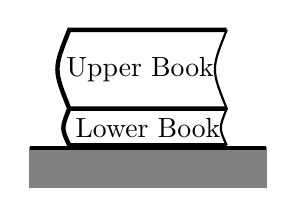
\begin{tikzpicture}
			\filldraw[gray] (0,0) rectangle (3,-0.5);
			\draw[ultra thick] (0,0) -- (3,0);
			\draw[ultra thick] (2.5,1pt) -- (0.5,1pt) .. controls (0.4,0.25) .. (0.5,0.5) -- (2.5,0.5) -- (0.5,0.5) .. controls (0.3,1) .. (0.5,1.5) -- (2.5,1.5);
			\draw[thick] (2.5,1pt) .. controls (2.4,0.25) .. (2.5,0.5) .. controls (2.3,1) .. (2.5,1.5);
			\node at (1.5,0.25) {Lower Book};
			\node at (1.4,1) {Upper Book};
		\end{tikzpicture}
	\end{center}
\end{textblock*}
\newpage
\begin{TeacherMargin}
\noindent At constant speed, $a_{A} = a_{B} = 0$, so $F^{net}_{A} = F^{net}_{B} = 0$. \\

\noindent Since the two stacked bricks are together in system A, the normal forces and forces of static friction between them are \ul{internal} to the forces. We only put external forces on free-body diagrams.
\begin{center}
	\begin{tikzpicture}
		\FBDbox{0,0}{0}{A}{A}
		\FBDvectorXY{Atcent}{0,1.2}{FNAT}
		\node[anchor=south] at (FNATtip) {$\vec{F}^{N}_{AT}$};
		\FBDvectorXY{Abcent}{0,-1.2}{FGAE}
		\node[anchor=north] at (FGAEtip) {$\vec{F}^{g}_{AE}$};
		\FBDvectorXY{Altq}{-1,0}{FKAT}
		\node[anchor=east] at (FKATtip) {$\vec{F}^{kf}_{AT}$};
		\FBDvectorXY{Albq}{-0.5,0}{FNAB}
		\node[anchor=east] at (FNABtip) {$\vec{F}^{N}_{AB}$};
		\FBDvectorXY{Arcent}{1.5,0}{FNAH}
		\node[anchor=west] at (FNAHtip) {$\vec{F}^{N}_{AH}$};
		\FBDbox{5,0}{0}{B}{B}
		\FBDvectorXY{Btcent}{0,0.6}{FNBT}
		\node[anchor=south] at (FNBTtip) {$\vec{F}^{N}_{BT}$};
		\FBDvectorXY{Bbcent}{0,-0.6}{FGBE}
		\node[anchor=north] at (FGBEtip) {$\vec{F}^{g}_{BE}$};
		\FBDvectorXY{Blcent}{-0.5,0}{FKBT}
		\node[anchor=east] at (FKBTtip) {$\vec{F}^{kf}_{BT}$};
		\FBDvectorXY{Brcent}{0.5,0}{FNBA}
		\node[anchor=west] at (FNBAtip) {$\vec{F}^{N}_{BA}$};
		\node[anchor=north] at (2.5,-0.5) {\parbox{2.5cm}{$\vec{F}^{N}_{AB}$ and $\vec{F}^{N}_{BA}$ are a third law pair.}};
		\node at (2.5,-3) {\Large$F^{N}_{AH} > F^{kf}_{AT} > F^{kf}_{BT} = F^{N}_{BA} = F^{N}_{AB}$};
		\draw[thick,<-] (0,-3.3) -- (-1.5,-4) node[anchor=north] {\parbox{4cm}{\centering 2nd
		\begin{align*}
			F^{net}_{Ax}&=F^{N}_{AH} - F^{kf}_{AT} - F^{N}_{AB} \\
			& = m_{A}a_{Ax}=0
		\end{align*}
		}};
		\draw[thick,<-] (1.75,-3.3) -- (1,-6) node[anchor=north] {\parbox{9cm}{\centering 2nd \& kinetic friction
		\[
		F^{kf}_{AT} = \mu_{k}F^{N}_{AT} = \mu_{k}m_{A}g = 2\mu_{k}m_{B}g = 2\mu_{k}F^{N}_{BT} = 2F^{kf}_{BT}
		\]
		}};
		\draw[thick,<-] (-0.73,-7) -- (-0.73,-8) node[anchor=north] {\parbox{1.75cm}{\centering 2nd law \\ $y$-direction system A}};
		\draw[thick,<-] (2.4,-7) -- (2.4,-8) node[anchor=north] {\parbox{1.75cm}{\centering 2nd law \\ $y$-direction system B}};
		\draw[thick,<-] (0.7,-7) -- (0.8,-8) node[anchor=north] {\parbox{1.75cm}{\centering A has 2 bricks}};
		\draw[thick,<-] (3.25,-3.3) -- (3.25,-4) node[anchor=north] {\parbox{4cm}{\centering 2nd
		\begin{align*}
			F^{net}_{Bx}&=F^{N}_{BA} - F^{kf}_{BT} \\
			& = m_{B}a_{Bx}=0
		\end{align*}
		}};
		\draw[thick,<-] (4.85,-3.3) -- (5.25,-4) node[anchor=north] {\parbox{4cm}{\centering 3rd}};
	\end{tikzpicture}
\end{center}
\end{TeacherMargin}
\begin{PresentSpace}
\vspace{-10pt}
\section*{S5-2: Moving Bricks I}
\vspace{-10pt}
\begin{itemize}
	\item Three identical bricks are pushed across a table at \textit{constant speed} as shown. The hand pushes horizontally. There is friction.
	\begin{center}
		\begin{tikzpicture}
			\node at (-0.75,1) {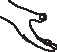
\includegraphics[scale=1.5]{KnightHand}};
			\draw[thick] (0,1) -- (2.5,1);
			\draw[ultra thick,blue] (0,0) rectangle (2.5,2);
			\draw[ultra thick,red] (2.56,0) rectangle (5.06,1);
			\node[anchor=south,blue] at (1.25,2) {A};
			\node[anchor=south,red] at (3.81,1) {B};
			\filldraw[gray] (-1,-0.06) rectangle (6,-0.56);
			\draw[ultra thick] (-1,-0.06) -- (6,-0.06);
			\node[anchor=south west] at (2.5,2) {\textit{Constant Speed}};
		\end{tikzpicture}
	\end{center}
	\item System A is the left (stacked) bricks, and system B is the right brick.
	\begin{itemize}
		\item Compare the \textit{net force} on system A to that on system B.
		\item Draw separate free-body diagrams for system A and system B.
		\item Identify all of the Newton's third law (action-reaction) force pairs.
		\item Rank the \textit{horizontal} forces by magnitude, from largest to smallest.
		\item Explain how you used Newton's laws.
	\end{itemize}
\end{itemize}
\end{PresentSpace}
\newpage
\begin{TeacherMargin}
\noindent With $\mu_{k}$ lower, the forces of friction decrease (by the same factor), therefore the boxes will now be accelerating together. Since $\vec{a}_{A} = \vec{a}_{B}$ and $m_{A} > m_{B}$, we know that $F^{net}_{A} > F^{net}_{B}$.
\begin{center}
	\begin{tikzpicture}
		\FBDbox{0,0}{0}{A}{A}
		\FBDvectorXY{Atcent}{0,1.2}{FNAT}
		\node[anchor=south] at (FNATtip) {$\vec{F}^{N}_{AT}$};
		\FBDvectorXY{Abcent}{0,-1.2}{FGAE}
		\node[anchor=north] at (FGAEtip) {$\vec{F}^{g}_{AE}$};
		\FBDvectorXY{Altq}{-0.6,0}{FKAT}
		\node[anchor=east] at (FKATtip) {$\vec{F}^{kf}_{AT}$};
		\FBDvectorXY{Albq}{-0.5,0}{FNAB}
		\node[anchor=east] at (FNABtip) {$\vec{F}^{N}_{AB}$};
		\FBDvectorXY{Arcent}{1.5,0}{FNAH}
		\node[anchor=west] at (FNAHtip) {$\vec{F}^{N}_{AH}$};
		\FBDbox{5,0}{0}{B}{B}
		\FBDvectorXY{Btcent}{0,0.6}{FNBT}
		\node[anchor=south] at (FNBTtip) {$\vec{F}^{N}_{BT}$};
		\FBDvectorXY{Bbcent}{0,-0.6}{FGBE}
		\node[anchor=north] at (FGBEtip) {$\vec{F}^{g}_{BE}$};
		\FBDvectorXY{Blcent}{-0.3,0}{FKBT}
		\node[anchor=east] at (FKBTtip) {$\vec{F}^{kf}_{BT}$};
		\FBDvectorXY{Brcent}{0.5,0}{FNBA}
		\node[anchor=west] at (FNBAtip) {$\vec{F}^{N}_{BA}$};
	\end{tikzpicture}
\end{center}
$F^{N}_{AB}$ and $F^{N}_{BA}$ do not change when the friction changes. The argument is a bit involved, and requires both the 2nd and 3rd laws.
\begin{align*}
	m_{B}a & = F^{net}_{Bx} \\
	& = F^{N}_{BA}-F^{kf}_{BT} \\
	& = F^{N}_{AB}-\mu_{k}m_{B}g \\
	m_{A}a & = F^{net}_{Ax} \\
	& = F^{N}_{AH}-F^{kf}_{AT}-F^{N}_{AB} \\
	& = F^{N}_{AH}-\mu_{k}m_{A}g-F^{N}_{AB} \\
	2m_{B}a & = F^{N}_{AH}-2\mu_{k}m_{B}g-F^{N}_{AB}
\end{align*}
The third and seventh lines together give us
\[
F^{N}_{AH}-2\mu_{k}m_{B}g-F^{N}_{AB} = 2(F^{N}_{AB}-\mu_{k}m_{B}g),
\]
and rearranging this and cancelling some terms gives us $F^{N}_{AH} = 3F^{N}_{AB}$, which has no dependence on $\mu_{k}$. \\

\noindent We need to know exactly how much $\mu_{k}$ changes in order to know if $F^{kf}_{AT}$ got smaller than $F^{N}_{AB}$, so we cannot completely rank the forces anymore. Other than that, the reasoning is the same as in S5-2:
\begin{align*}
	F^{N}_{AH} \overset{\text{2nd}}{>} F^{N}_{AB} & \overset{\text{3rd}}{=} F^{N}_{BA} \overset{\text{2nd}}{>} F^{kf}_{BT}, & F^{N}_{AH} \overset{\text{2nd}}{>} F^{kf}_{AT} & \underset{\text{\& kf}}{\overset{\text{2nd}}{>}} F^{kf}_{BT}.
\end{align*}
\end{TeacherMargin}
\begin{PresentSpace}
\vspace{-10pt}
\section*{S5-3: Moving Bricks II}
\vspace{-10pt}
\begin{itemize}
	\item The hand still pushes horizontally, but the coefficient of friction is less than it was in S5-2.
	\begin{center}
		\begin{tikzpicture}
			\node at (-0.75,1) {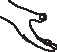
\includegraphics[scale=1.5]{KnightHand}};
			\draw[thick] (0,1) -- (2.5,1);
			\draw[ultra thick,blue] (0,0) rectangle (2.5,2);
			\draw[ultra thick,red] (2.56,0) rectangle (5.06,1);
			\node[anchor=south,blue] at (1.25,2) {A};
			\node[anchor=south,red] at (3.81,1) {B};
			\filldraw[gray] (-1,-0.06) rectangle (6,-0.56);
			\draw[ultra thick] (-1,-0.06) -- (6,-0.06);
			\node[anchor=south west] at (2.5,2) {\parbox{5cm}{\centering Hand pushes with \textit{same force} as in S5-2.}};
			\node[anchor=north] at (2.5,-0.56) {Coefficient of friction \textit{less than} in S5-2.};
		\end{tikzpicture}
	\end{center}
	\begin{itemize}
		\item How does the motion of the blocks change, if at all?
		\item Compare the \textit{net force} on system A to that on system B.
		\item Draw separate free-body diagrams for system A and system B.
		\item Rank the \textit{horizontal} forces by magnitude, from largest to smallest. (Is it possible to rank the horizontal forces \textit{completely}?)
		\item Explain how you used Newton's laws.
	\end{itemize}
\end{itemize}
\end{PresentSpace}
\newpage
\begin{TeacherMargin}
\noindent First, you do not need to assume that $m_{1} > m_{2}$ for this setup to work. You can imagine that, in the frictionless case, this system would certainly start to slide, and low friction cases should approach the outcome of the frictionless version. \\

\noindent If the system accelerates from rest, it will start to slide left (sliding right, uphill for $m_{1}$, makes no physical sense in this situation), so kinetic friction will point to the right, along the surface.
\begin{center}
	\begin{tikzpicture}
		\FBDbox{0,0}{45}{MO}{$m_{1}$}
		\FBDvectorMA{MOrtq}{0.25}{45}{FKOS}
		\node[anchor=south] at (FKOStip) {$\vec{F}^{kf}_{1S}$};
		\FBDvectorMA{MOrbq}{0.75}{45}{FTOR}
		\node[anchor=south] at (FTORtip) {$\vec{F}^{T}_{1R}$};
		\FBDvectorMA{MOtcent}{1.5}{135}{FNOS}
		\node[anchor=south] at (FNOStip) {$\vec{F}^{N}_{1S}$};
		\FBDvectorXY{MObl}{0,{-1.5*sqrt(2)}}{FGOE}
		\node[anchor=north] at (FGOEtip) {$\vec{F}^{g}_{1E}$};
		\FBDbox{4,0}{0}{MT}{$m_{2}$}
		\FBDvectorXY{MTrcent}{0.25,0}{FKTS}
		\node[anchor=west] at (FKTStip) {$\vec{F}^{kf}_{2S}$};
		\FBDvectorXY{MTlcent}{-0.75,0}{FNTR}
		\node[anchor=east] at (FNTRtip) {$\vec{F}^{T}_{2R}$};
		\FBDvectorXY{MTtcent}{0,1.5}{FNTS}
		\node[anchor=south] at (FNTStip) {$\vec{F}^{N}_{2S}$};
		\FBDvectorXY{MTbcent}{0,-1.5}{FGTS}
		\node[anchor=north] at (FGTStip) {$\vec{F}^{g}_{2E}$};
	\end{tikzpicture}
\end{center}
\textbf{There are no 3rd law pairs!} \\
The two tensions are equal ($F^{T}_{1R} = F^{T}_{2R}$), but not directly because of the third law. Third law pairs must be between two directly interacting objects (in the notation, the subscripts should reverse: $\vec{F}_{AB}$ versus $\vec{F}_{BA}$). Third law pairs must also be equal and opposite ($\vec{F}_{AB}=-\vec{F}_{BA}$), but $\vec{F}^{T}_{1R}$ and $\vec{F}^{T}_{2R}$ do not point in opposite directions.
\begin{itemize}
	\item $\vec{F}^{T}_{1R}$ is in a 3rd law pair with $\vec{F}^{T}_{R1}$ (the force of tension from $m_{1}$ on the rope).
	\item $\vec{F}^{T}_{2R}$ is in a 3rd law pair with $\vec{F}^{T}_{R2}$ (the force of tension from $m_{2}$ on the rope).
	\item $F^{T}_{R2}=F^{T}_{R1}$ due to two assumptions: (i) an ideal (massless and inextensible) rope, and (ii) an ideal pulley.
	\begin{enumerate}[(i)]
		\item keeps the tensions constant throughout lengths of free rope
		\item keeps the tensions equal across the pulley
	\end{enumerate}
	\item In summary: $F^{T}_{1R} \overset{\text{3rd}}{=} F^{T}_{R1} \underset{\text{(ii)}}{\overset{\text{(i)}}{=}} F^{T}_{R2} \overset{\text{3rd}}{=} F^{T}_{2R}$.
\end{itemize}
\end{TeacherMargin}
\begin{PresentSpace}
\vspace{-10pt}
\section*{S5-4: Angled Ramp}
\vspace{-10pt}
\begin{itemize}
	\item Draw separate free-body diagrams for both objects in the situation below.
	\begin{itemize}
		\item Assume there is friction between all blocks and surfaces.
		\item Assume each system accelerates from rest.
	\end{itemize}
	\item Identify all of the Newton's third law (action-reaction) force pairs.
\end{itemize}
\begin{center}
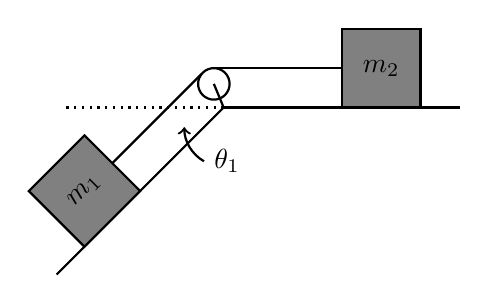
\begin{tikzpicture}
	\begin{scope}
		\draw[thick] (0,0) -- (3,0);
		\draw[thick,color=black,fill=gray] (1.5,0) rectangle (2.5,1);
		\node at (2,0.5) {$m_{2}$};
		\draw[thick] (-0.1,0.5) -- (1.5,0.5);
	\end{scope}
	\draw[thick,dotted] (0,0) -- (-2,0);
	\draw[thick,<-] (-0.5,-0.25) arc (180:240:0.5) node[anchor=west] {$\theta_{1}$};
	\draw[thick,rotate=112.5] (0.325,0) circle (0.2);
	\draw[thick,rotate=112.5] (0,0) -- (0.325,0);
	\begin{scope}[rotate=45]
		\draw[thick] (0,0) -- (-3,0);
		\draw[thick,color=black,fill=gray] (-1.5,0) rectangle (-2.5,1);
		\node[rotate=45] at (-2,0.5) {$m_{1}$};
		\draw[thick] (0.1,0.5) -- (-1.5,0.5);
	\end{scope}
\end{tikzpicture}
\end{center}
\end{PresentSpace}
\newpage
\begin{TeacherMargin}
\noindent Let us call the rope that goes around the pulley R$_{1}$, and the rope pulled by the hand R$_{2}$. I am comfortable giving the entire rope around the pulley a single label, as using the ideal string and ideal pulley assumptions allow me to keep the tension constant in the rope. In a more general circumstance, I might give different names to the parts of the rope separated by the pulley. \\
\textbf{Counting Forces}
\begin{itemize}
	\item Each block has one long-range force (gravity).
	\item $m_{1}$ has 3 contact forces. The rope R$_{1}$ is pulling it (that's one, tension) and it is touching $m_{2}$ (that's two, normal and friction).
	\item $m_{2}$ has 6 contact forces. There are two ropes pulling it, and it touches both the surface below (two more forces) and $m_{1}$ above (two more forces).
\end{itemize}
\textbf{Free-Body Diagrams} \\
If the system accelerates from rest, the top block must be pulled left, and the bottom block must be pulled right. First, this tells us that the net force on $m_{1}$ must be to the left, and the net force on $m_{2}$ must be to the right. Furthermore, based on the relative motion between the two boxes, the friction on $m_{1}$ by $m_{2}$ must point right, and the friction on $m_{2}$ by $m_{1}$ must point left.
\begin{center}
	\begin{tikzpicture}
		\FBDbox{0,0}{0}{MTbox}{$m_{2}$}
		\FBDvectorXY{MTboxblq}{0,-2.25}{FGTE}
		\node[anchor=north] at (FGTEtip) {$\vec{F}^{g}_{2E}$};
		\FBDvectorXY{MTboxbrq}{0,-0.75}{FNTO}
		\node[anchor=north] at (FNTOtip) {$\vec{F}^{N}_{21}$};
		\FBDvectorXY{MTboxtcent}{0,3}{FNTS}
		\node[anchor=south] at (FNTStip) {$\vec{F}^{N}_{2S}$};
		\FBDvectorXY{MTboxltq}{-0.5,0}{FKTO}
		\node[anchor=south east] at (FKTOtip) {$\vec{F}^{kf}_{21}$};
		\FBDvectorXY{MTboxlcent}{-1,0}{FTTRO}
		\node[anchor=south east] at (FTTROtip) {$\vec{F}^{T}_{2R_{1}}$};
		\FBDvectorXY{MTboxlbq}{-1.5,0}{FKTS}
		\node[anchor=east] at (FKTStip) {$\vec{F}^{kf}_{2S}$};
		\FBDvectorXY{MTboxrcent}{3.9,0}{FTTRT}
		\node[anchor=west] at (FTTRTtip) {$\vec{F}^{T}_{2R_{2}}$};
		\FBDbox{3,2}{0}{MObox}{$m_{1}$}
		\FBDvectorXY{MOboxbcent}{0,-0.75}{FGOE}
		\node[anchor=north] at (FGOEtip) {$\vec{F}^{g}_{1E}$};
		\FBDvectorXY{MOboxtcent}{0,0.75}{FNOT}
		\node[anchor=south] at (FNOTtip) {$\vec{F}^{N}_{12}$};
		\FBDvectorXY{MOboxrcent}{0.5,0}{FKOT}
		\node[anchor=west] at (FKOTtip) {$\vec{F}^{kf}_{12}$};
		\FBDvectorXY{MOboxlcent}{-0.8,0}{FTORO}
		\node[anchor=east] at (FTOROtip) {$\vec{F}^{T}_{1R_{1}}$};
	\end{tikzpicture}
\end{center}
\textbf{3rd Law Pairs}
\begin{itemize}
	\item $\vec{F}^{N}_{12}=-\vec{F}^{N}_{21}$
	\item $\vec{F}^{kf}_{12}=-\vec{F}^{kf}_{21}$
\end{itemize}
Even though $\vec{F}^{T}_{1R_{1}}$ and $\vec{F}^{T}_{2R_{1}}$ are equal in magnitude, they are not a 3rd law pair. They point in the same direction, and these forces are not part of an interaction that is directly between the two masses (the rope acts as an intermediary).
\end{TeacherMargin}
\begin{PresentSpace}
\vspace{-10pt}
\section*{S5-5: Horizontal Pulley}
\vspace{-10pt}
\begin{itemize}
	\item Draw separate free-body diagrams for both objects in the situation below.
	\begin{itemize}
		\item Assume there is friction between all blocks and surfaces.
		\item Assume the strings and the pulley are ideal.
		\item Assume each system accelerates from rest.
	\end{itemize}
	\item Identify all of the Newton's third law (action-reaction) force pairs.
\end{itemize}
\begin{center}
\begin{tikzpicture}
	\draw[thick] (0,2) -- (0,0) -- (7,0);
	\draw[ultra thick,color=black,fill=gray] (1,1) circle (0.5);
	\draw[thick] (0,1) -- (1,1);
	\draw[thick] (1,1.5) -- (4.5,1.5);
	\draw[thick] (1,0.5) -- (2.5,0.5);
	\draw[thick,color=black,fill=gray] (2.5,0) rectangle (5.5,1);
	\node at (4,0.5) {$m_{2}$};
	\draw[thick,color=black,fill=gray] (4.5,1) rectangle (5.5,2);
	\node at (5,1.5) {$m_{1}$};
	\draw[thick] (5.5,0.5) -- (7,0.5);
	\node[shift={(7,0.75)},rotate=240] at (0,0) {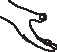
\includegraphics{KnightHand}};
\end{tikzpicture}
\end{center}
\end{PresentSpace}
\newpage
\begin{TeacherMargin}

\end{TeacherMargin}
\begin{PresentSpace}
\section*{Main Ideas}
\begin{itemize}
	\item Newton's 3rd law of motion can be used to relate the forces acting on \textit{different} objects or systems.
\end{itemize}
\end{PresentSpace}
\end{document}